\section{Algorytm Gaussa-Legendre'a}

Algorytm Gaussa-Legendre'a jest aktualnie jednym z najszybciej zbiegających algorytmów używanych do wyliczania liczb $\pi$. Został wyprowadzony na podstawie prac Carla Friedricha Gaussa oraz Adrien-Marie Legendre na podstawie współczesnych algorytmów do mnożenia i pierwiastkowania.Jest on, niestety, bardzo wymagający pamięciowo. Poniżej prezentujemy implementację tego algorytmu\cite{gausse2}:

\begin{lstlisting}[language=ps]
function gauss_legrendre (max):
    a = 1
    b = 1 / sqrt(2)
    t = 1 / 4
    p = 1
    i = 0
    while i <= max:
        an = (a + b) / 2
        b = sqrt(a * b)
        t = t - p * (a - an) * (a - an)
        p = 2 * p
        a = an
    
    return (a + b) * (a + b) / (4 * t)
\end{lstlisting}

\subsection{Wyniki}

Metoda Gaussa-Legrendre'a okazała się zbiegać do implementacji bibliotecznej funkcji \verb+pi()+ z języka \verb+Julia+ wyjątkowo szybko, bo już w 11 iteracji kwadrat błędu maszynowo był równy zeru, co widać na Wykresie~\ref{gauss-errorq}.

\begin{figure}[!h]
    \centering
    \renewcommand{\figurename}{Wykres}
    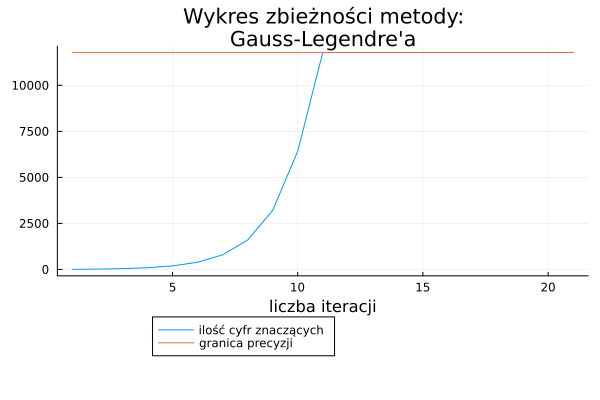
\includegraphics[width=0.7\textwidth]{../prog/gauss_legendre_log_error.png}
    \caption{Wykres logarytmu dziesiętnego z błędu względnego dla przybliżenia $\pi$ za pomocą algorytmu Gaussa-Legendre'a.}
    \label{gauss-error}
\end{figure}

Eksperymentalne obliczenia rzędu zbieżności tej metody jedynie potwierdzają wyższą zbieżność tego algorytmu niż w przypadku innych opisanych metod. Dla precyzji wynoszącej 16 069 bitów obliczenia na podstawie dzielenia błędu $(n+1)$-ego wyrazu przez kwadrat błędu $n$-tego wyrazu nie dają konkretnych wyników przez zbyt szybkie dążenie tej metody do $\pi$. W literaturze metoda ta jest określana jako zbieżna kwadratowo \cite{gausse-smth}.

\begin{figure}[!h]
    \centering
    \renewcommand{\figurename}{Wykres}
    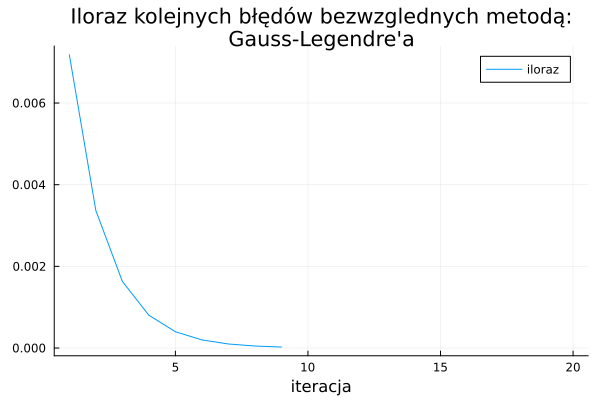
\includegraphics[width=0.7\textwidth]{../prog/gauss_legendre_error_ratio.png}
    \caption{Wykres ilorazu błędów względnych wyrazu $n+1$ i $n$ dla algorytmu Gassa-Legrendre'a.}
    \label{gauss-convergence}
\end{figure}